%---Linda

\subsection{Methods}\label{GPS:subsec:methods}

The aim of this report is to measure the ice velocity of the two glaciers which calculated on different points on the glaciers. 
The points are consitently given by the mass balance stakes as a reference point to the last years.
The velocity will be calculated by the position difference of the stakes as a function of time.

Regarding to the results of the previous years, it is given that the ice velocity for the glaciers Tellbreen and Blekumbreen is less then one meter.
The position measurements during the fieldwork are made with GPS. 
The general used GPS system has only an accurancy in the order of meters.
By correcting the measurement data with the data from the base station, it is posssible to have a more accurate positioning to the order of millimeters \citep{UGPS}. This method is named dGPS.
\medskip

% GPS theory:
The GPS signal is broadcast with two certain frequencies L1 and L2 which belongs two different services.
The transmisson signals with L1 and L2 are the carrier component, which is one component of the Global Navigation Satellite System (GNSS) structure the GPS receivers are using.
In the GNSS there are 24 operational plus some redundant stallites available.
To reach the satellites the signal has to go through the different atmospheric layers \citep{curcherdgps}, because the orbit of the satellites is approximately in 20000 km \citep{Trprocess}.
\medskip

There are five different GNSS constellations GPS, GLONASS, QZSS, COMPASS and Galileo they can used while the GPS measurements.
The Real-time Kinematic (RTK) positioning has the concept to remove errors based on the comparison to the base station.
When the position of the satellite is known, the position of the receiver is calculated by trilateration based on the measured distance between receiver and each satellite.
The position of the satellite is broadcast as a ephemerides, which is a specific positioning.
For reducong the errors by different sources the receiver need a additional source with precise positions, clock offsets and goog correction of atmosphic disturbances. 
Differential positioning is used to reduce the errors by orbit and atmosphere, which are similar for both receiver as long as the distance in between is not too long. 
The Carrier phase is used for the measurements because it has a smaller wavenegth than the Pseudorandom Noise (PRN) code signal.
To measure the difference in the phase of the received signal and the phase of an equivalent signal is taken which is generated from the receiver’s oscillator or clock \citep{Trprocess}.
\medskip

The errors from the GPS measurements that are corrected by the dGPS method are correlated in time and space.
So the identified errors can assumed to be the same at the reciever as at the base station.
The disturbances can be distingushed, because the position of the base station is very well known.
The realistion of the GPS error correlation between two recievers with a specific distance can be defined as a baseline.
Also a time correlation is meaningful, because there is always a time delay in the data tranfer possible.
Possible disturbances can caused by satellite clock errors, ephermeris errors, tropospheric errors (variation of the speed of electromagnetic radiation), ionospheric errors (dependent on signal frequency, elevation angle and the total electron content). 
There are also the reciever noise and multipath as a uncorreleted error source between the two recievers \citep{UGPS}.
For further information it is to recommend to read in the referenced book.
\medskip

% methods and usings in the field
The GPS measurements have been done with the Trimble differential Global Navigation Satellite System (GNSS). 
The measured parameters were the northing and easting as well as the elevation.
The setting during our measurements inculded the receiver Trimble R4, the controller Trimble TCS2 and a carbon pole to mount the receiver proberly next to the stake (see figure).
During the operation of the measuremts we followed exact the description in section 2 and 3 in \cite{Trquickstart}. 
The recommended Fast Static survey method is used.
The used coordinate system is the Universal Transversal Mercator (UTM) for the zone 33x with WGS 1984 date \citep{Trquickstart}. 
\medskip

The accurancy of the dGPS depends on the distance to the base station and differs between the horizontal and the vertical component.
For the Fast Static method the horizontal accuracy is $ \pm $ 3 mm + 0.1 ppm and vertical $ \pm $ 3.5 + 0.4 ppm  \citep{Trquickstart}.
The accurancy can reached because the coordinates of the base station are well known. 
So the disturbances by the atmosphere during the measuring time can be corrected, while the measured coordinates are compare on every timestep defined by the GPS time.. 
The further steps of the post processing is explanined in the next section \ref{processing}.
We also did two measurements at the same stake on two different days to see how the results are effected.
\medskip

The duration for our measurments with the GPS receiver was at least 15 minutes. 
We had to made choice with a trade off between the quality of the result and the total number of measurements to measure all stakes at least one time. 
With a longer measurement time the statistical fluctuations are better avereaged out.
\medskip

The analysis in this report is made with python.

\subsection{Setup} \label{GPS:subsec:setup}

The setup for our measurments is specifed by a specific guideline to insure that the measurements are consistent during the whole fieldwork.
The receiver on the carbon pole has to be positioned on the top on the stake as far as possible. 
To determine the uncertainty from a tilted stake, it is necessary to measure the inclination of the stake as well as the direction of inclination with the compass.
The snow depth is measured with the probe which has a centimeter scale on it.
With snow depth and the antenna height the actual height over the ice surface is known. 
When the stake is already melted out too high, it is necessary to put the pole with the rover next to the stake. 
In this case the poles has to be positioned northwards of the stake so that the correction is only to the northing component, which makes the calculation easier. 
Also the distance from the receiver to stake is measured.
These two differenr setups are shown in photographs in the figure \ref{GPS:fig:setup}.

\begin{figure}[H]
	\centering
	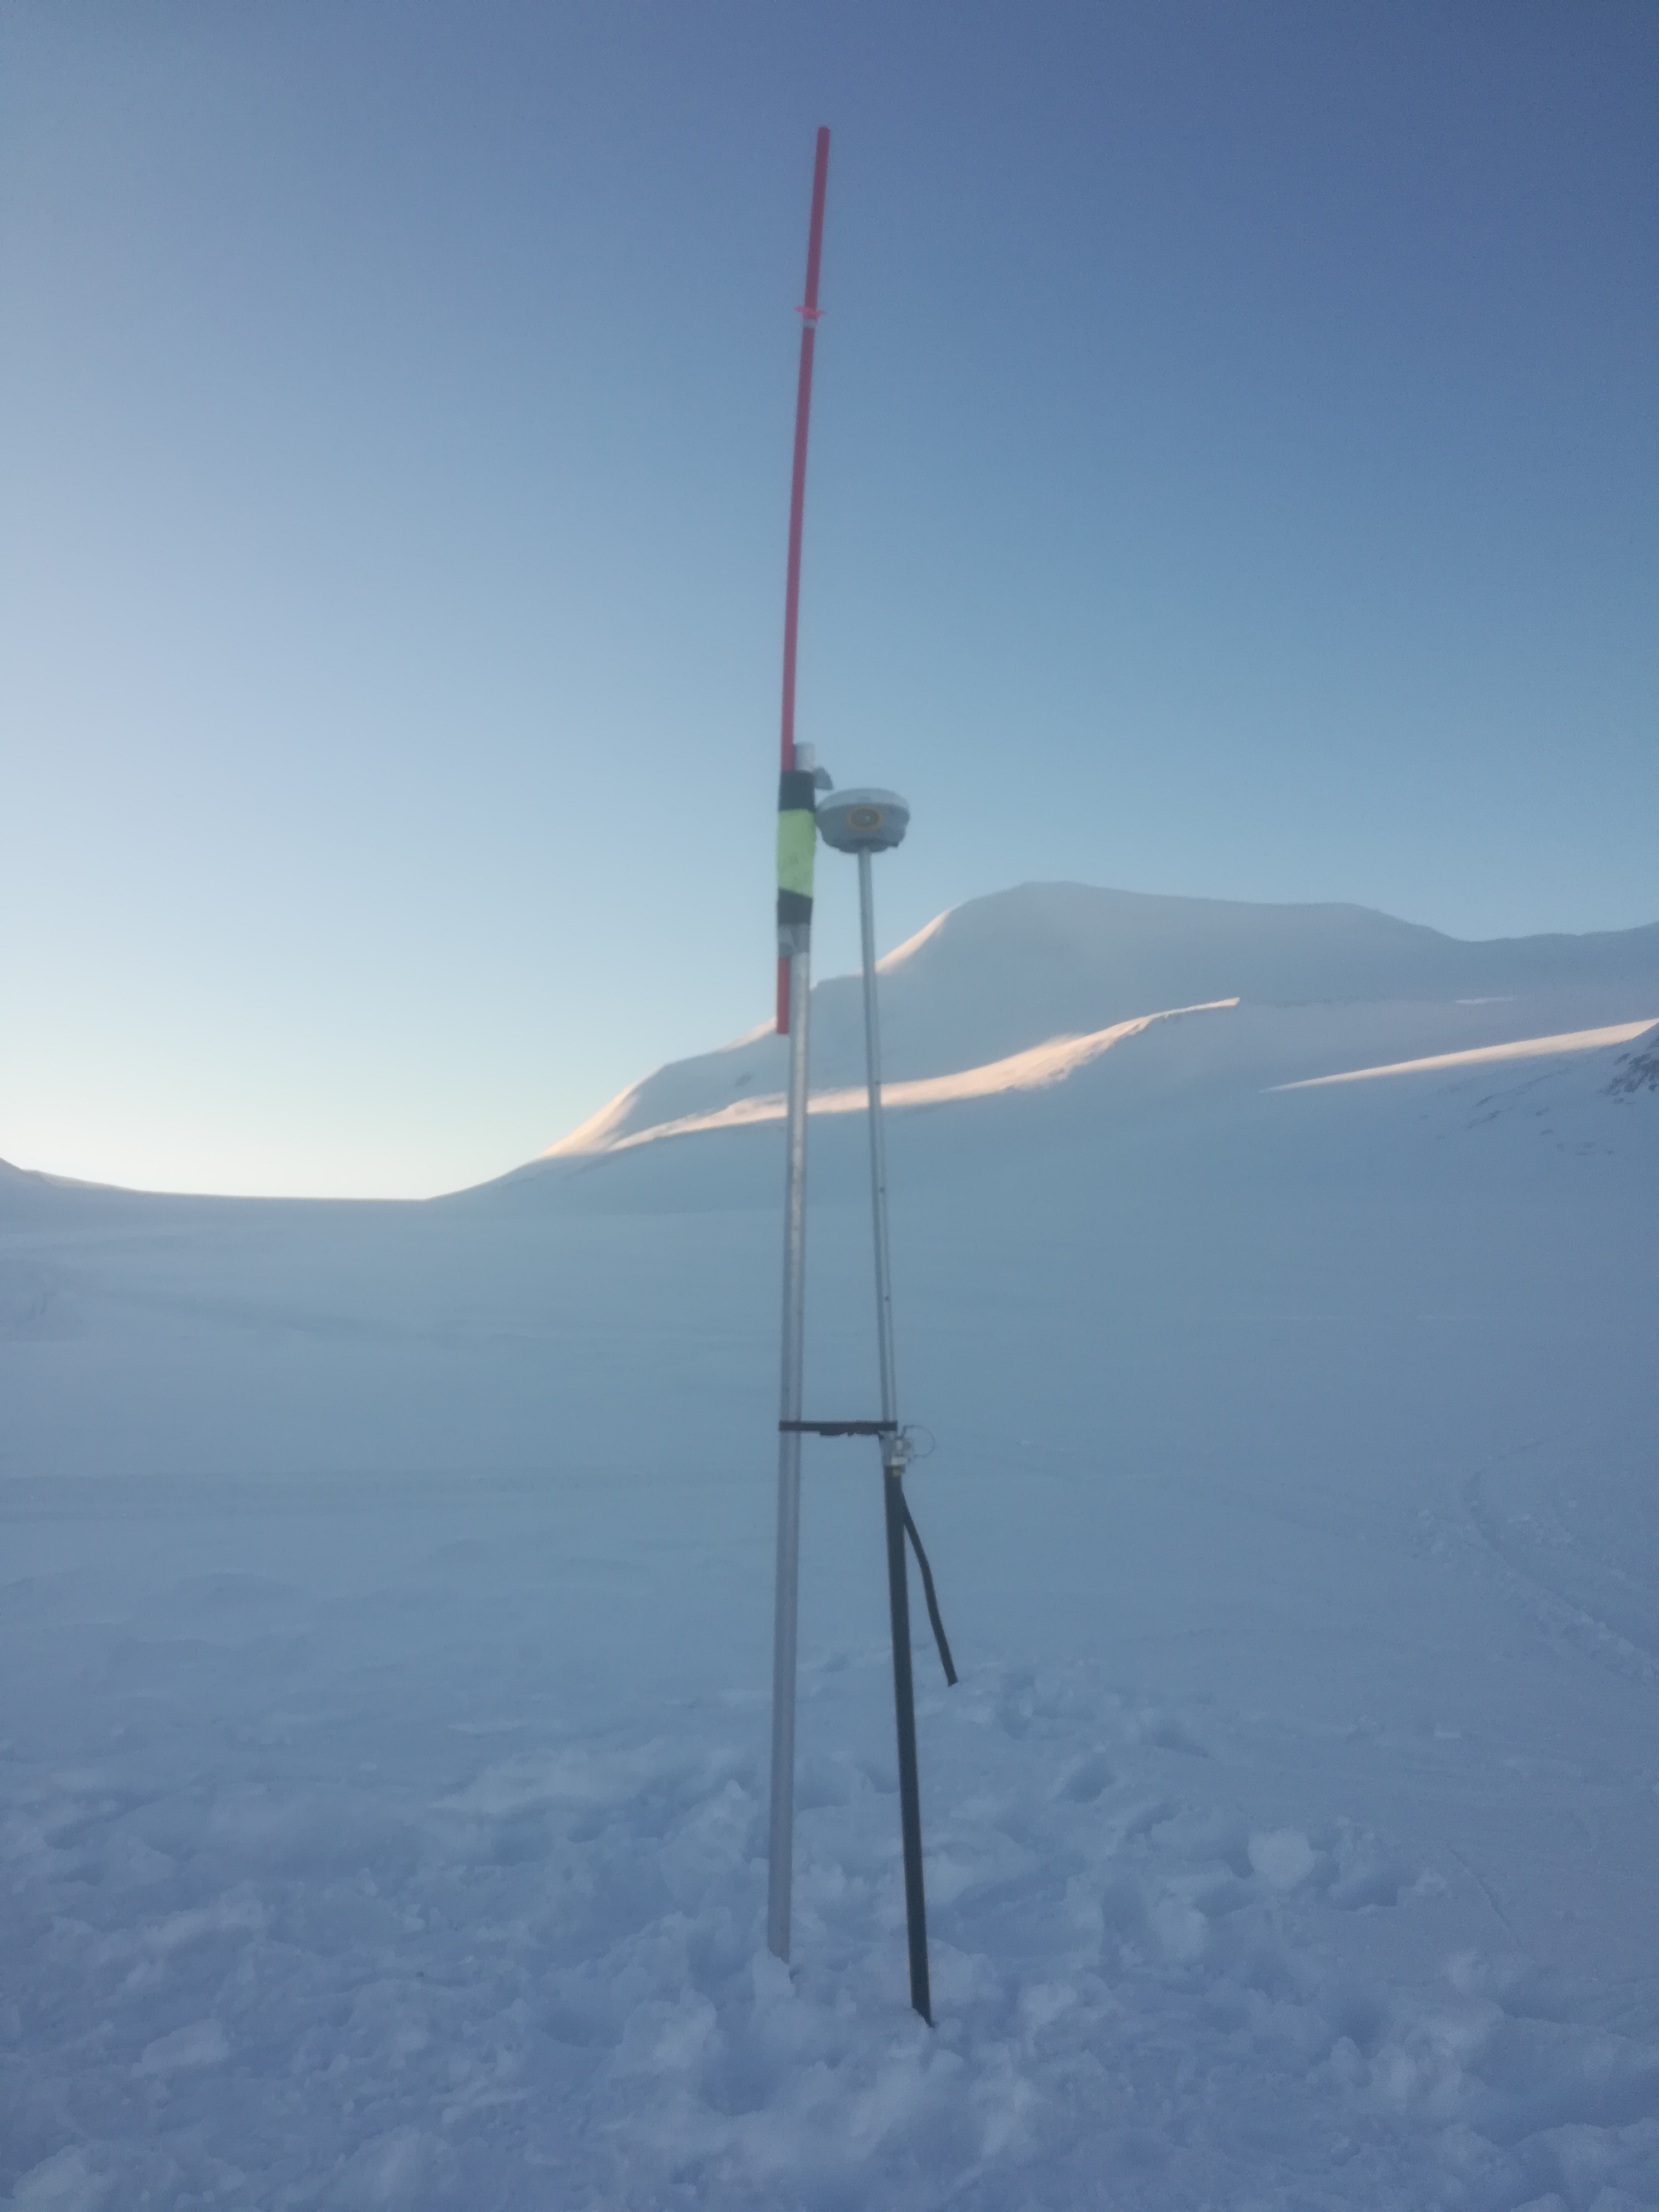
\includegraphics[width=0.48\linewidth]{./figs/pictures/GPS_setup.jpg}
	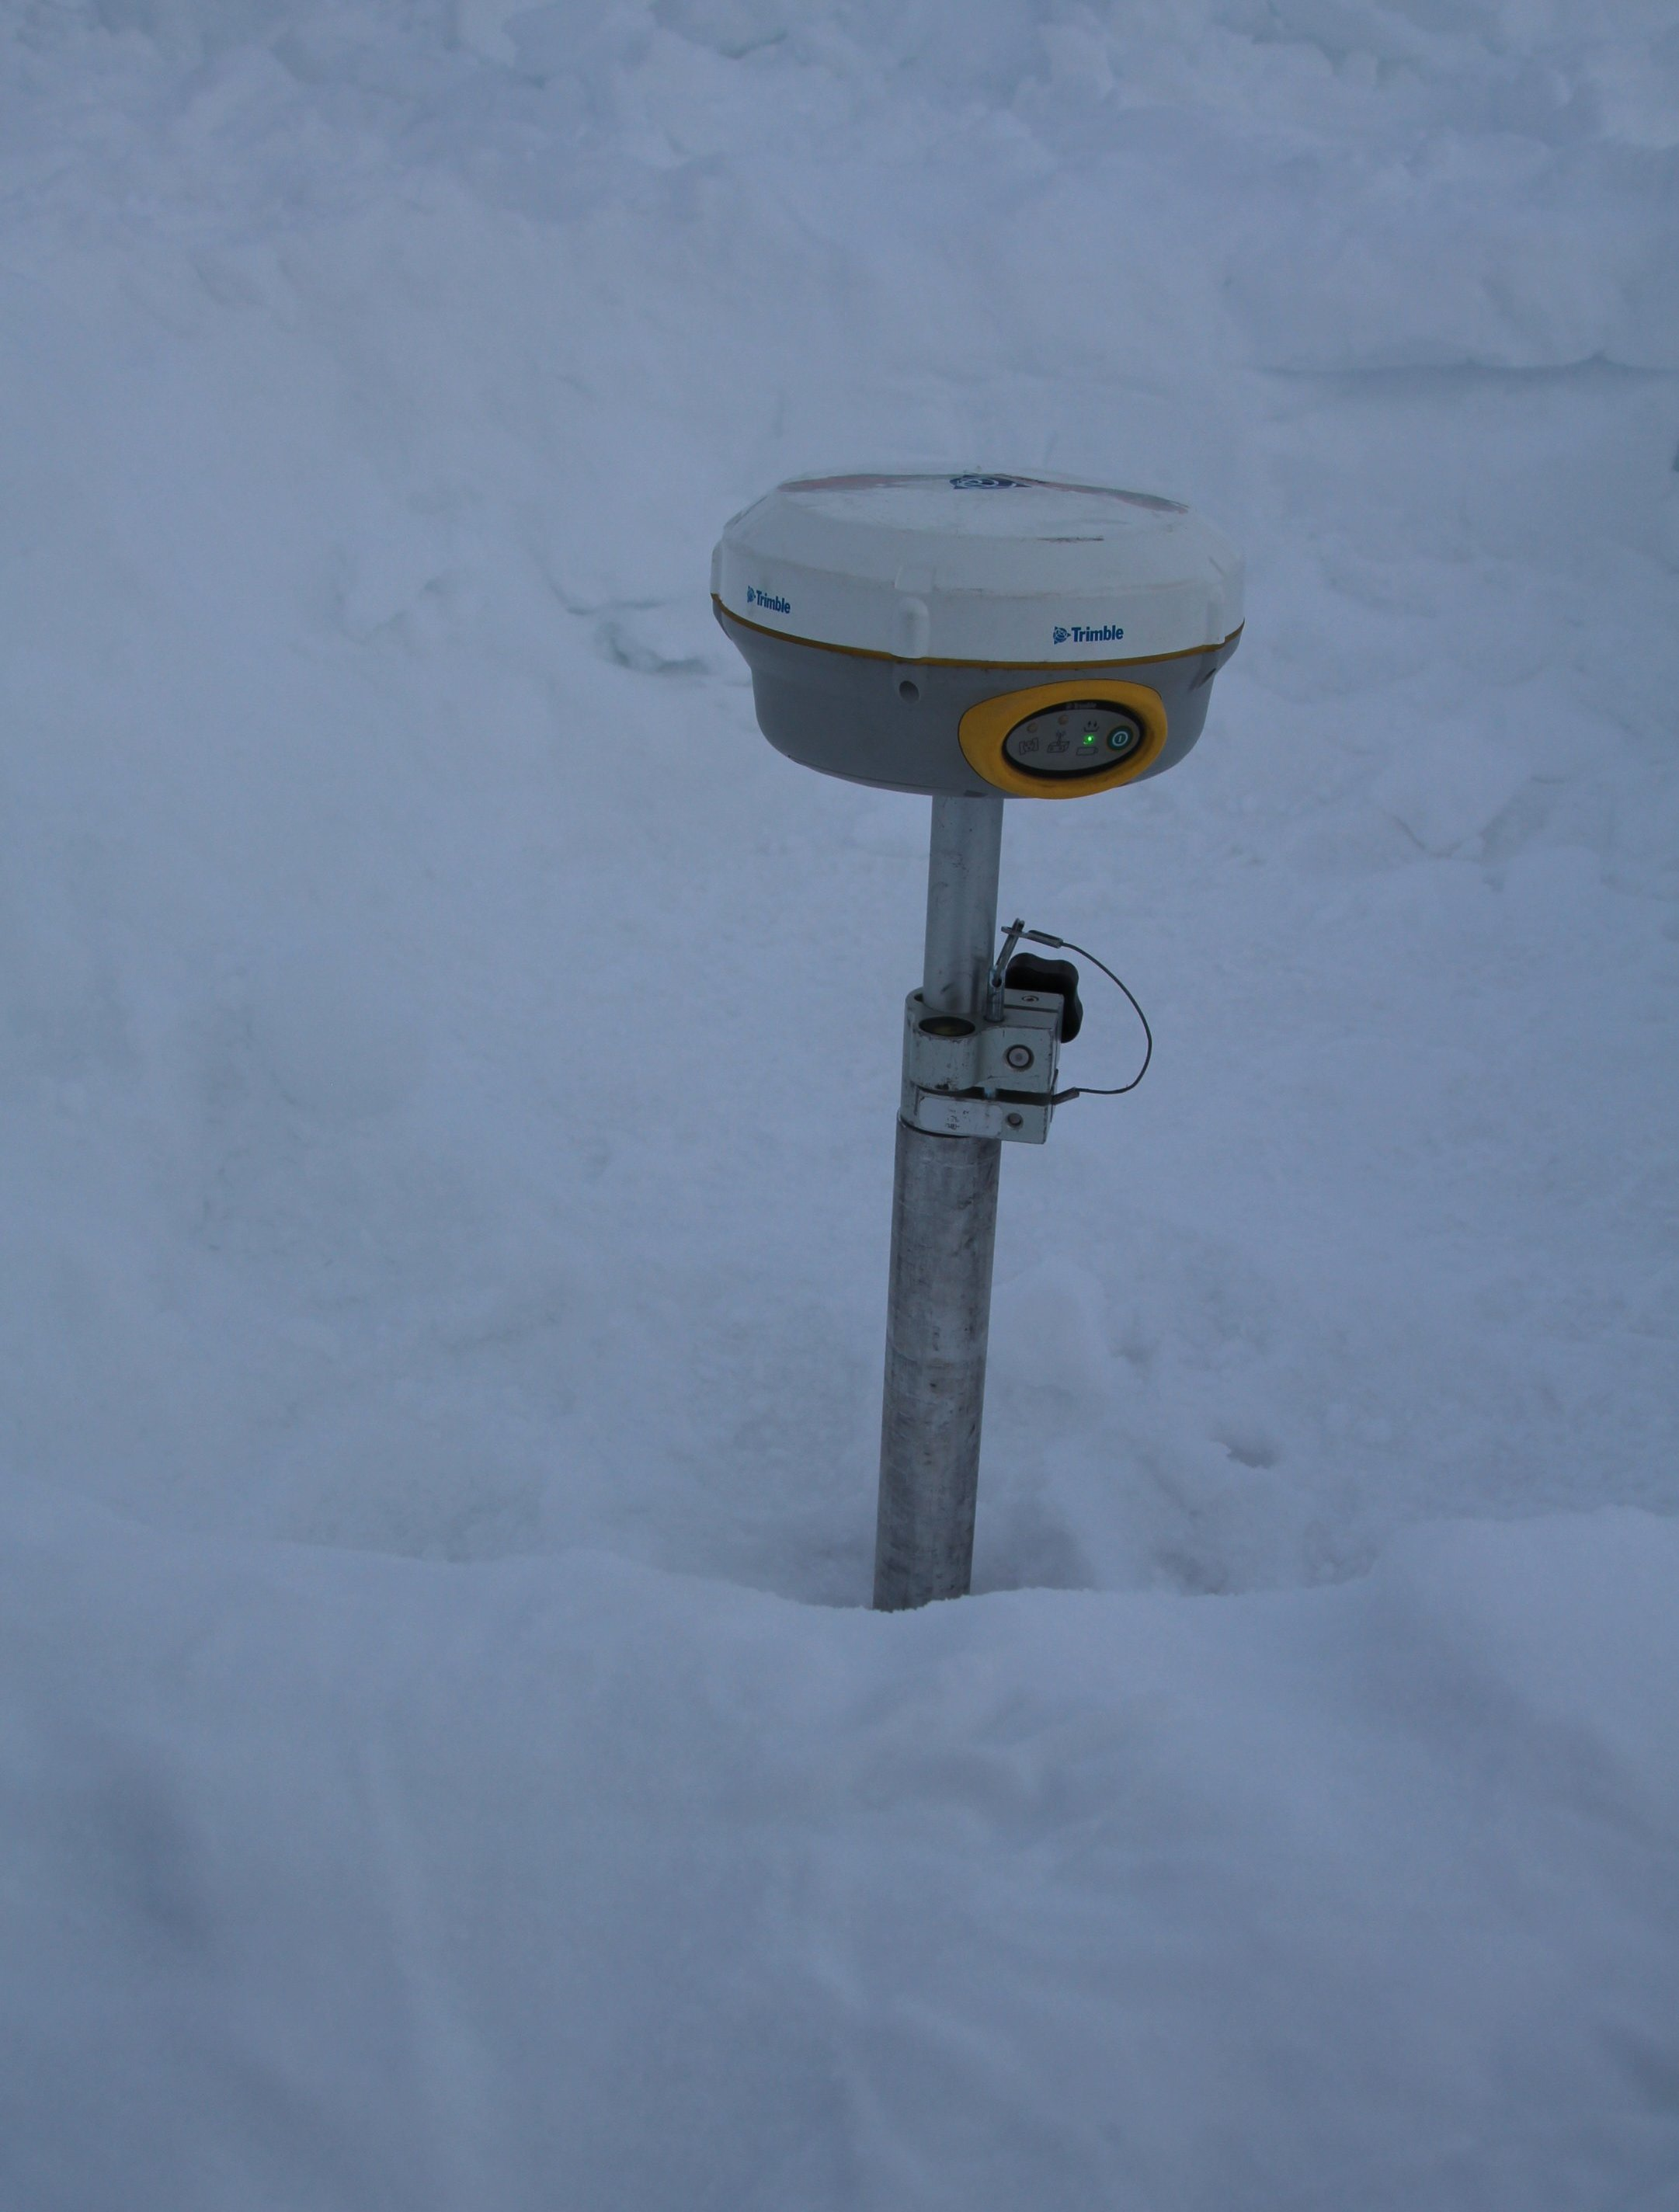
\includegraphics[width=0.485\linewidth]{./figs/pictures/setup_ontop.JPG}
	\caption{Setup while the GPS measurement next to the stake (left) and on top of the stake (right).}
	\label{GPS:fig:setup}
\end{figure}
